\documentclass[12pt,a4paper]{article}

% ─── Page Layout ───────────────────────────────────────────────────────────────
\usepackage[a4paper, margin=0.8in, headheight=14pt]{geometry}

% ─── Fonts (XeLaTeX) ───────────────────────────────────────────────────────────
\usepackage{fontspec}
\usepackage{unicode-math}
\setmainfont{TeX Gyre Pagella}
\setmonofont[Scale=0.88]{TeX Gyre Cursor}
\setmathfont{Latin Modern Math}

% ─── Packages ──────────────────────────────────────────────────────────────────
\usepackage{xcolor}
\usepackage{colortbl}
\usepackage{titlesec}
\usepackage{enumitem}
\usepackage{tabularx}
\usepackage{booktabs}
\usepackage{array}
\usepackage{amsmath}
\usepackage{tikz}
\usetikzlibrary{shapes.geometric, arrows.meta, positioning, calc, fit, decorations.pathreplacing}
\usepackage{tcolorbox}
\tcbuselibrary{skins, breakable}
\usepackage{hyperref}
\usepackage{fancyhdr}
\usepackage{graphicx}
\usepackage{microtype}
\hyphenpenalty=10000
\exhyphenpenalty=10000
\sloppy
\usepackage{caption}
\usepackage{setspace}
\usepackage{multirow}
\usepackage{tocloft}

% ─── Q&A helper ────────────────────────────────────────────────────────────────
\newcommand{\Q}[1]{\textbf{#1}\par\noindent\ignorespaces}

% ─── Colour Palette ────────────────────────────────────────────────────────────
\definecolor{myred}{RGB}{196,30,58}
\definecolor{mydark}{RGB}{30,30,50}
\definecolor{mygreen}{RGB}{14,120,80}
\definecolor{myteal}{RGB}{0,130,140}
\definecolor{myamber}{RGB}{180,100,0}
\definecolor{mypurple}{RGB}{100,30,160}
\definecolor{mygray}{RGB}{246,247,249}
\definecolor{mgframe}{RGB}{180,185,200}
\definecolor{watermark}{RGB}{145,150,170}
\definecolor{hdrred}{RGB}{250,232,235}
\definecolor{hdrgreen}{RGB}{220,244,233}
\definecolor{hdrteal}{RGB}{220,242,244}
\definecolor{hdramber}{RGB}{253,242,215}
\definecolor{hdrpurple}{RGB}{238,228,255}
\definecolor{hdrgray}{RGB}{238,240,245}
\definecolor{rowalt}{RGB}{250,251,253}

% ─── Section Formatting ────────────────────────────────────────────────────────
\titleformat{\section}
  {\large\bfseries\color{myred}}{\thesection.}{0.5em}{}
  [\vspace{1pt}{\color{myred}\rule{\linewidth}{0.8pt}}]
\titleformat{\subsection}
  {\normalsize\bfseries\color{myteal}}{\thesubsection}{0.5em}{}
\titlespacing*{\section}{0pt}{18pt}{7pt}
\titlespacing*{\subsection}{0pt}{11pt}{4pt}

% ─── Paragraph ─────────────────────────────────────────────────────────────────
\setlength{\parindent}{0pt}
\setlength{\parskip}{4pt}

% ─── TOC Styling ───────────────────────────────────────────────────────────────
\renewcommand{\cfttoctitlefont}{\large\bfseries\color{myred}}
\renewcommand{\cftaftertoctitle}{\par\noindent{\color{myred}\rule{\linewidth}{0.8pt}}}
\setlength{\cftbeforetoctitleskip}{0pt}
\setlength{\cftaftertoctitleskip}{6pt}
\renewcommand{\cftsecfont}{\normalsize\bfseries\color{mydark}}
\renewcommand{\cftsecpagefont}{\normalsize\bfseries\color{mydark}}
\renewcommand{\cftsecleader}{\cftdotfill{\cftdotsep}}
\setlength{\cftbeforesecskip}{7pt}
\renewcommand{\cftsubsecfont}{\small\color{mydark}}
\renewcommand{\cftsubsecpagefont}{\small\color{mydark}}
\setlength{\cftbeforesubsecskip}{3pt}
\setlength{\cftsubsecindent}{1.4em}

% ─── Table helpers ─────────────────────────────────────────────────────────────
\renewcommand{\arraystretch}{1.45}
\setlength{\tabcolsep}{6pt}
\arrayrulecolor{mydark}
\newcolumntype{B}[1]{>{\small\bfseries\raggedright\arraybackslash}m{#1}}
\newcolumntype{Y}{>{\small\raggedright\arraybackslash}X}
\renewcommand{\tabularxcolumn}[1]{m{#1}}

% ─── Header / Footer ───────────────────────────────────────────────────────────
\pagestyle{fancy}
\fancyhf{}
\fancyhead[L]{\small\color{myred}\textbf{PE-EC703A}\;\color{mydark}--- Embedded System}
\fancyhead[R]{\small\color{myteal}\textbf{Module 1 Notes}}
\fancyfoot[C]{\small\color{mydark}\thepage}
\fancyfoot[R]{\small\color{watermark}\textit{\copyright\ Biraj}}
\renewcommand{\headrulewidth}{0.5pt}
\renewcommand{\footrulewidth}{0.3pt}

% ─── Hyperref ──────────────────────────────────────────────────────────────────
\hypersetup{
  colorlinks=true, linkcolor=myteal, urlcolor=myteal,
  pdfauthor={Biraj Sarkar},
  pdftitle={PE-EC703A --- Module 1 Notes}
}

% ─── tcolorbox styles ──────────────────────────────────────────────────────────
\tcbset{
  tikzbox/.style={
    colback=mygray, colframe=mgframe, boxrule=0.6pt, arc=4pt,
    left=8pt, right=8pt, top=6pt, bottom=6pt,
    colbacktitle=mgframe, coltitle=mydark,
    fonttitle=\small\bfseries
  },
  defbox/.style={
    colback=hdrgreen, colframe=mygreen, boxrule=0.8pt, arc=4pt,
    left=9pt, right=9pt, top=6pt, bottom=6pt,
    colbacktitle=mygreen, coltitle=white,
    fonttitle=\small\bfseries
  },
  formulabox/.style={
    colback=hdrteal, colframe=myteal, boxrule=0.8pt, arc=4pt,
    left=9pt, right=9pt, top=7pt, bottom=7pt,
    colbacktitle=myteal, coltitle=white,
    fonttitle=\small\bfseries
  },
  examplebox/.style={
    colback=hdramber, colframe=myamber, boxrule=0.8pt, arc=4pt,
    left=9pt, right=9pt, top=6pt, bottom=6pt,
    colbacktitle=myamber, coltitle=white,
    fonttitle=\small\bfseries
  },
  masonbox/.style={
    colback=hdrpurple, colframe=mypurple, boxrule=0.8pt, arc=4pt,
    left=9pt, right=9pt, top=6pt, bottom=6pt,
    colbacktitle=mypurple, coltitle=white,
    fonttitle=\small\bfseries
  },
  exambox/.style={
    colback=hdrpurple, colframe=mypurple, boxrule=1pt, arc=5pt,
    left=10pt, right=10pt, top=8pt, bottom=8pt,
    colbacktitle=mypurple, coltitle=white,
    fonttitle=\bfseries,
    breakable, title after break={\textbf{Frequently Asked / Viva Questions (contd.)}}}
}
% Make all boxes breakable across pages
\tcbset{breakable}

% ─── TikZ styles ───────────────────────────────────────────────────────────────
\tikzset{
  block/.style={rectangle, draw=myteal, fill=hdrteal,
    text width=2.4cm, align=center, minimum height=0.95cm,
    font=\small, rounded corners=3pt, line width=0.7pt},
  redblock/.style={rectangle, draw=myred, fill=hdrred,
    text width=2.4cm, align=center, minimum height=0.95cm,
    font=\small, rounded corners=3pt, line width=0.7pt},
  netnode/.style={rectangle, draw=myteal, fill=hdrteal,
    text width=1.5cm, align=center, minimum height=0.8cm,
    font=\small, rounded corners=3pt, line width=0.7pt},
  sumjunc/.style={circle, draw=myamber, fill=hdramber,
    minimum size=0.62cm, font=\small, line width=0.8pt},
  snode/.style={circle, draw=mypurple, fill=hdrpurple,
    minimum size=0.55cm, font=\footnotesize, line width=0.7pt},
  arrow/.style={-Stealth, thick, color=mydark},
  redarrow/.style={-Stealth, thick, color=myred},
  line/.style={thick, color=mydark}
}

% ═══════════════════════════════════════════════════════════════════════════════
\begin{document}
% ═══════════════════════════════════════════════════════════════════════════════

\begin{center}
  {\LARGE\bfseries\color{myred} PE-EC703A --- Embedded System}\\[5pt]
  {\normalsize\color{mydark} Semester VII \quad$\bullet$\quad 3L:0T:0P \quad$\bullet$\quad 3 Credits}\\[3pt]
  {\normalsize\color{myteal}\textbf{Module 1 Exam Notes: Overview of Embedded Systems}}\\[3pt]
  {\small\color{mydark} CGEC \;$|$\; B.Tech ECE (2023--27) \;$|$\; \textit{Biraj Sarkar}}
\end{center}
\vspace{2pt}
\noindent{\color{myred}\rule{\linewidth}{1.5pt}}
\vspace{2pt}

\hypersetup{linkcolor=mydark}
\tableofcontents
\hypersetup{linkcolor=myteal}
\newpage

% ===============================================================================
\section{What is an Embedded System?}
% ===============================================================================

An embedded system is a combination of hardware and software designed to perform a specific dedicated function within a larger system. Unlike general-purpose computers, embedded systems are purpose-built and optimized for a particular task.

\begin{tcolorbox}[defbox, title={\textbf{Embedded System --- Definition}}]
An \textbf{embedded system} is a dedicated computing system that is tightly integrated into the device it controls. It consists of a microprocessor or microcontroller, memory, I/O interfaces, and software (firmware) designed to perform one or more specific tasks --- often with real-time constraints and limited resources (power, memory, processing speed).
\end{tcolorbox}

\subsection{Key Characteristics}
\begin{itemize}[leftmargin=*, itemsep=3pt]
  \item \textbf{Single-function:} Designed to perform a specific task (e.g., engine control, temperature monitoring).
  \item \textbf{Real-time operation:} Must respond to events within strict time deadlines.
  \item \textbf{Resource-constrained:} Limited memory (RAM/ROM), processing power, and energy budget.
  \item \textbf{Reliability:} Must operate continuously and correctly, often without human intervention.
  \item \textbf{Embedded into a product:} The computing part is hidden inside a larger product (e.g., washing machine, car).
\end{itemize}

% ===============================================================================
\section{Embedded Processor in a System}
% ===============================================================================

\begin{tcolorbox}[defbox, title={\textbf{Embedded Processor}}]
An \textbf{embedded processor} is the central computational element of an embedded system. It can be a \textbf{microprocessor} (requires external memory and peripherals), a \textbf{microcontroller} (integrates CPU, memory, and peripherals on a single chip), a \textbf{DSP} (optimized for signal processing), or an \textbf{FPGA/ASIC} (for high-speed, custom logic).
\end{tcolorbox}

\subsection{Types of Embedded Processors}

\par\noindent
{\renewcommand{\arraystretch}{1.6}%
\begin{tabularx}{\linewidth}{|B{3.0cm}|Y|Y|}
\hline
\textbf{Processor Type} & \textbf{Description} & \textbf{Examples / Use} \\
\hline
\textbf{Microcontroller (MCU)} & CPU + RAM + ROM + I/O on one chip & 8051, PIC, ARM Cortex-M, AVR \\
\hline
\textbf{Microprocessor (MPU)} & CPU only; needs external memory and peripherals & Intel 8086, ARM Cortex-A \\
\hline
\textbf{DSP Processor} & Optimized for multiply-accumulate (MAC) operations & TMS320, SHARC \\
\hline
\textbf{FPGA / ASIC} & Reconfigurable / custom-designed logic fabric & Xilinx, Intel Altera \\
\hline
\textbf{SoC} & Entire system (CPU + GPU + memory + I/O) on one die & Qualcomm Snapdragon, Raspberry Pi SoC \\
\hline
\end{tabularx}}

% ===============================================================================
\section{Components of an Embedded System}
% ===============================================================================

An embedded system is made up of several hardware and software components that work together.

\begin{tcolorbox}[tikzbox, title={Components of an Embedded System}]
\centering
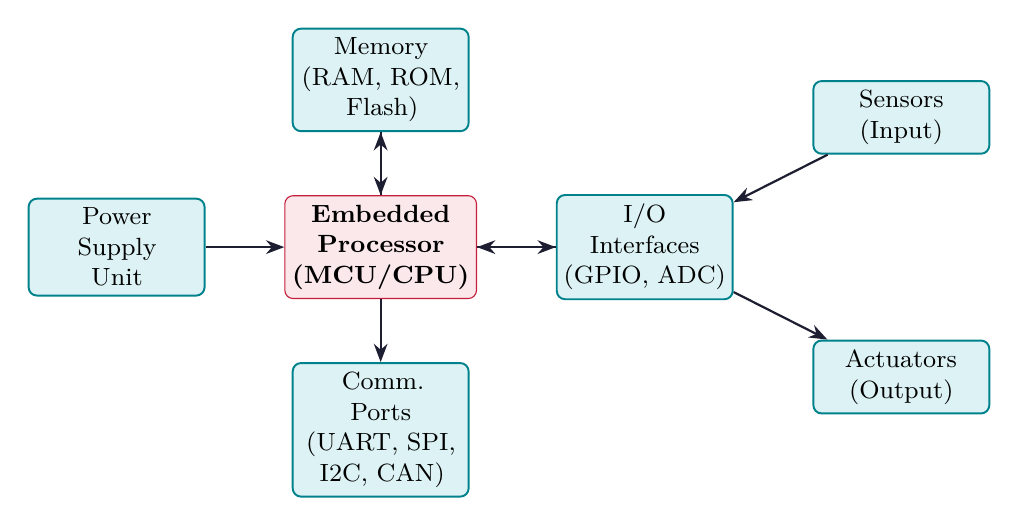
\begin{tikzpicture}[node distance=0.4cm and 0.7cm,
  sblock/.style={rectangle, draw=myteal, fill=hdrteal, text width=2.0cm,
    align=center, minimum height=0.85cm, font=\small,
    rounded corners=3pt, line width=0.7pt}]
  % Central MCU
  \node[rectangle, draw=myred, fill=hdrred, text width=2.2cm, align=center,
    minimum height=1.0cm, font=\small\bfseries, rounded corners=3pt] (mcu) {Embedded\\Processor\\(MCU/CPU)};
  % Surrounding blocks
  \node[sblock, above=0.8cm of mcu] (mem) {Memory\\(RAM, ROM,\\Flash)};
  \node[sblock, right=1.0cm of mcu] (io) {I/O\\Interfaces\\(GPIO, ADC)};
  \node[sblock, below=0.8cm of mcu] (comm) {Comm.\\Ports\\(UART, SPI,\\I2C, CAN)};
  \node[sblock, left=1.0cm of mcu] (pwr) {Power\\Supply\\Unit};
  \node[sblock, above right=0.5cm and 1.0cm of io] (sens) {Sensors\\(Input)};
  \node[sblock, below right=0.5cm and 1.0cm of io] (act) {Actuators\\(Output)};

  \draw[arrow] (mcu) -- (mem);
  \draw[arrow] (mem) -- (mcu);
  \draw[arrow] (mcu) -- (io);
  \draw[arrow] (io) -- (mcu);
  \draw[arrow] (mcu) -- (comm);
  \draw[arrow] (pwr) -- (mcu);
  \draw[arrow] (sens) -- (io);
  \draw[arrow] (io) -- (act);
\end{tikzpicture}
\end{tcolorbox}

\subsection{Hardware Components}
\begin{itemize}[leftmargin=*, itemsep=3pt]
  \item \textbf{Processor Core:} The CPU that fetches, decodes, and executes instructions.
  \item \textbf{Memory:}
    \begin{itemize}[itemsep=2pt]
      \item \textbf{ROM / Flash:} Stores firmware (non-volatile, permanent program code).
      \item \textbf{RAM:} Temporary storage for variables and stack (volatile).
      \item \textbf{EEPROM:} Non-volatile, electrically erasable; stores configuration data.
    \end{itemize}
  \item \textbf{I/O Ports:} Digital GPIO, analog ADC/DAC inputs and outputs.
  \item \textbf{Communication Interfaces:} UART, SPI, I2C, CAN, USB.
  \item \textbf{Timers/Counters:} Generate time delays, PWM signals, and measure frequency.
  \item \textbf{Clock Source:} Crystal oscillator, RC oscillator, or PLL --- drives system timing.
  \item \textbf{Power Supply:} Regulated DC supply (often 3.3V or 5V); may include battery management.
\end{itemize}

\subsection{Software Components}
\begin{itemize}[leftmargin=*, itemsep=3pt]
  \item \textbf{Boot Loader:} First code that runs on power-up; initializes hardware and loads the main program.
  \item \textbf{Operating System / RTOS:} Manages tasks, scheduling, memory, and I/O (optional; may be bare-metal).
  \item \textbf{Device Drivers:} Software layer that abstracts hardware peripherals (UART driver, SPI driver, etc.).
  \item \textbf{Application Software:} The main program implementing the embedded task.
  \item \textbf{Middleware:} Protocol stacks (TCP/IP, USB), file systems, or GUI libraries.
\end{itemize}

% ===============================================================================
\section{Embedded Software in a System}
% ===============================================================================

\begin{tcolorbox}[defbox, title={\textbf{Embedded Software (Firmware)}}]
\textbf{Embedded software}, also called \textbf{firmware}, is the software permanently programmed into the non-volatile memory (ROM/Flash) of an embedded system. It directly controls hardware and implements the system's application logic. Unlike desktop software, it cannot be easily updated by the end-user.
\end{tcolorbox}

\subsection{Levels of Embedded Software}

The embedded software stack has distinct layers, each serving a different purpose:

\begin{tcolorbox}[tikzbox, title={Embedded Software Layered Architecture}]
\centering
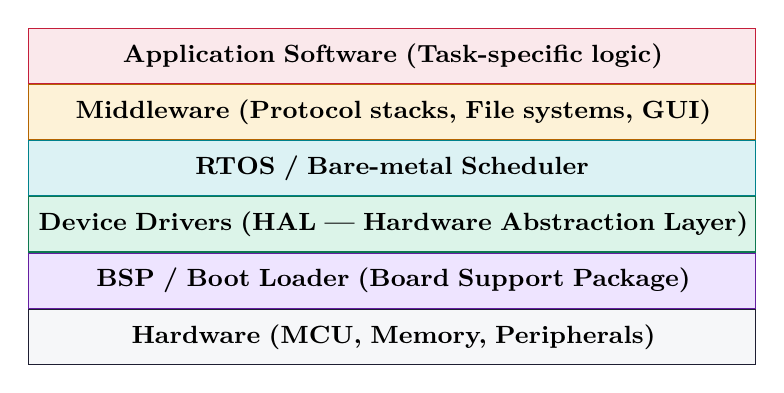
\begin{tikzpicture}[node distance=0.0cm]
  \node[rectangle, draw=myred, fill=hdrred, text width=9cm, align=center,
    minimum height=0.7cm, font=\small\bfseries] (app) {Application Software (Task-specific logic)};
  \node[rectangle, draw=myamber, fill=hdramber, text width=9cm, align=center,
    minimum height=0.7cm, font=\small\bfseries, below=0.0cm of app] (mid) {Middleware (Protocol stacks, File systems, GUI)};
  \node[rectangle, draw=myteal, fill=hdrteal, text width=9cm, align=center,
    minimum height=0.7cm, font=\small\bfseries, below=0.0cm of mid] (rtos) {RTOS / Bare-metal Scheduler};
  \node[rectangle, draw=mygreen, fill=hdrgreen, text width=9cm, align=center,
    minimum height=0.7cm, font=\small\bfseries, below=0.0cm of rtos] (drv) {Device Drivers (HAL --- Hardware Abstraction Layer)};
  \node[rectangle, draw=mypurple, fill=hdrpurple, text width=9cm, align=center,
    minimum height=0.7cm, font=\small\bfseries, below=0.0cm of drv] (bsp) {BSP / Boot Loader (Board Support Package)};
  \node[rectangle, draw=mydark, fill=mygray, text width=9cm, align=center,
    minimum height=0.7cm, font=\small\bfseries, below=0.0cm of bsp] (hw) {Hardware (MCU, Memory, Peripherals)};
\end{tikzpicture}
\end{tcolorbox}

\subsection{Brief Introduction to Embedded Software Categories}
\begin{itemize}[leftmargin=*, itemsep=3pt]
  \item \textbf{Programming Languages Used:} Assembly language (for low-level hardware control), C (most common for embedded), and C++ (for OOP in embedded, limited use).
  \item \textbf{Bare-metal Programming:} No OS; application code runs directly on hardware. Used in simple, resource-constrained systems.
  \item \textbf{RTOS-based Programming:} Uses a real-time OS for multi-task management. Used when multiple functions must run concurrently with timing guarantees.
  \item \textbf{Firmware Updates (OTA):} Modern embedded systems support Over-The-Air updates to patch firmware without physical access.
\end{itemize}

% ===============================================================================
\section{Design Process in Embedded Systems}
% ===============================================================================

The development of an embedded system follows a structured design process to ensure the product meets functional, real-time, power, and cost requirements.

\begin{tcolorbox}[tikzbox, title={Embedded System Design Process Flow}]
\centering
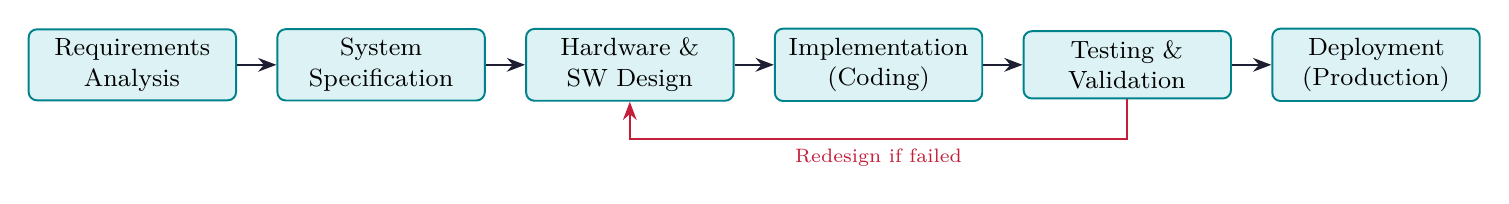
\begin{tikzpicture}[node distance=0.3cm and 0.5cm,
  sblock/.style={rectangle, draw=myteal, fill=hdrteal, text width=2.4cm,
    align=center, minimum height=0.8cm, font=\small, rounded corners=3pt, line width=0.7pt}]
  \node[sblock] (req) {Requirements\\Analysis};
  \node[sblock, right=0.5cm of req] (spec) {System\\Specification};
  \node[sblock, right=0.5cm of spec] (des) {Hardware \&\\SW Design};
  \node[sblock, right=0.5cm of des] (impl) {Implementation\\(Coding)};
  \node[sblock, right=0.5cm of impl] (test) {Testing \&\\Validation};
  \node[sblock, right=0.5cm of test] (dep) {Deployment\\(Production)};

  \draw[arrow] (req) -- (spec);
  \draw[arrow] (spec) -- (des);
  \draw[arrow] (des) -- (impl);
  \draw[arrow] (impl) -- (test);
  \draw[arrow] (test) -- (dep);
  % Feedback arrow
  \draw[redarrow] (test.south) -- ++(0,-0.5) -| (des.south)
    node[pos=0.25, below, font=\scriptsize\color{myred}] {Redesign if failed};
\end{tikzpicture}
\end{tcolorbox}

\subsection{Design Steps Explained}

\begin{enumerate}[label=\textbf{\arabic*.}, leftmargin=*, itemsep=4pt]
  \item \textbf{Requirements Analysis:} Identify what the system must do --- functional requirements (what it does), non-functional requirements (speed, power, cost, size, reliability). Example: ``Control motor speed based on temperature sensor; respond within 10 ms.''
  \item \textbf{System Specification:} Define architecture --- partitioning between hardware and software. Specify processor type, memory size, I/O count, communication protocol, and OS requirements.
  \item \textbf{Hardware Design:} Schematic design (circuit), PCB layout, selection of MCU/processor, memory, power supply IC, and peripheral components.
  \item \textbf{Software Design:} Algorithm design, data flow diagrams, state machines. Choosing programming language (C/Assembly), RTOS selection, ISR design.
  \item \textbf{Implementation:} Writing firmware code (in C or Assembly). Cross-compilation using a host computer to generate binary for the target MCU. Flashing the binary into MCU flash memory.
  \item \textbf{Testing and Validation:} Unit testing (individual modules), integration testing, hardware-in-the-loop (HIL) testing, real-time performance testing. Verify timing deadlines, power consumption, and EMI compliance.
  \item \textbf{Deployment:} Mass production, product integration, final firmware version locked, field testing.
\end{enumerate}

\subsection{Hardware--Software Co-design}

Modern embedded design uses \textbf{hardware--software co-design} --- HW and SW are developed concurrently and their partitioning is optimized to meet cost and performance targets.

\par\noindent
{\renewcommand{\arraystretch}{1.55}%
\begin{tabularx}{\linewidth}{|B{3.2cm}|Y|Y|}
\hline
\textbf{Aspect} & \textbf{Hardware Implementation} & \textbf{Software Implementation} \\
\hline
\textbf{Speed} & Very fast (gate-level logic) & Slower (instruction-by-instruction) \\
\hline
\textbf{Flexibility} & Fixed after fabrication & Easily modified (just reflash) \\
\hline
\textbf{Cost} & High NRE (Non-Recurring Engineering) & Low cost for updates \\
\hline
\textbf{Example} & CRC calculation in FPGA & CRC computed in C function \\
\hline
\end{tabularx}}

% ===============================================================================
% MANDATORY QUICK REVISION PAGE
% ===============================================================================
\newpage
\begin{center}
  {\large\bfseries\color{myred} Quick Revision --- Module 1}\\[3pt]
  {\small\color{mydark} Overview of Embedded Systems $|$ PE-EC703A}
\end{center}
\noindent{\color{myred}\rule{\linewidth}{1.2pt}}
\vspace{4pt}

\begin{tcolorbox}[formulabox, title={\textbf{Key Formulas at a Glance}}]
\renewcommand{\arraystretch}{1.3}
\begin{tabularx}{\linewidth}{B{4.5cm} X}
System Clock Period & $T = \displaystyle\frac{1}{f_{clk}}$ \quad (e.g., 12 MHz clock $\Rightarrow T = 83.3\,\text{ns}$) \\[4pt]
Instruction Cycle & $t_{inst} = \frac{N_{cycles}}{f_{clk}}$ \quad ($N_{cycles}$ = machine cycles per instruction) \\[4pt]
Power Dissipation & $P = C \cdot V_{DD}^2 \cdot f$ \quad (dynamic power in CMOS logic) \\[4pt]
Response Time Deadline & $t_{response} \leq t_{deadline}$ \quad (real-time constraint; must always hold)
\end{tabularx}
\end{tcolorbox}

\begin{tcolorbox}[defbox, title={\textbf{One-Line Definitions}}]
\begin{itemize}[leftmargin=*, itemsep=2.5pt, topsep=0pt]
  \item \textbf{Embedded System:} Dedicated computing system embedded inside a product to perform a specific function with real-time constraints.
  \item \textbf{Firmware:} Software permanently stored in ROM/Flash; directly controls hardware.
  \item \textbf{MCU:} Microcontroller Unit --- CPU, RAM, ROM, and peripherals all on one chip.
  \item \textbf{MPU:} Microprocessor Unit --- CPU only; needs external support chips.
  \item \textbf{RTOS:} Real-Time Operating System --- guarantees task completion within hard time deadlines.
  \item \textbf{HAL:} Hardware Abstraction Layer --- software interface that hides hardware details from application code.
  \item \textbf{BSP:} Board Support Package --- low-level software that initializes specific hardware board peripherals.
  \item \textbf{Bare-metal:} Programming directly on hardware without an operating system.
  \item \textbf{Cross-compiler:} A compiler running on a host PC that generates code for a different target architecture (e.g., ARM).
  \item \textbf{Hard real-time:} System where missing a deadline causes catastrophic failure (e.g., airbag control).
  \item \textbf{Soft real-time:} System where missing a deadline degrades performance but is not fatal (e.g., video streaming).
\end{itemize}
\end{tcolorbox}

\begin{tcolorbox}[exambox, title={\textbf{Frequently Asked / Viva Questions}}]
\begin{enumerate}[topsep=0pt, label=\textbf{Q\arabic*.}, itemsep=5pt]
  \item \Q{Define an embedded system. How does it differ from a general-purpose computer?}
    An embedded system is a dedicated computing unit integrated into a product to perform a specific function (e.g., car ABS controller). A general-purpose computer (PC) can run any program. Embedded systems are resource-constrained, single-function, and often real-time.
  \item \Q{What are the key components of an embedded system?}
    \begin{itemize}[leftmargin=*, itemsep=1pt, topsep=2pt]
      \item Processor (MCU/MPU), Memory (RAM/ROM/Flash), I/O Interfaces
      \item Communication ports (UART, SPI, I2C, CAN), Timers, Clock source, Power supply
    \end{itemize}
  \item \Q{What is the difference between a microprocessor and a microcontroller?}
    A \textbf{microprocessor} contains only the CPU; it needs external RAM, ROM, and peripherals. A \textbf{microcontroller} integrates CPU, RAM, ROM, and peripherals on a single chip --- lower cost, smaller size, less power.
  \item \Q{What is firmware? Where is it stored?}
    Firmware is the embedded software (program code) that directly controls hardware. It is stored in \textbf{non-volatile memory} --- ROM, Flash, or EEPROM --- so it persists after power-off.
  \item \Q{What is meant by real-time in embedded systems?}
    Real-time means the system must complete its tasks within guaranteed time limits (deadlines). In \textbf{hard real-time} systems, missing a deadline causes system failure. In \textbf{soft real-time}, performance degrades but operation continues.
  \item \Q{List the steps in the embedded system design process.}
    Requirements analysis $\to$ System specification $\to$ HW \& SW design $\to$ Implementation (coding) $\to$ Testing and validation $\to$ Deployment.
  \item \Q{What is hardware--software co-design?}
    It is the simultaneous design of hardware and software components, optimizing their partitioning to meet cost, performance, and power goals. Functions can be implemented in either HW (faster, fixed) or SW (flexible, cheaper to modify).
  \item \Q{What is a BSP (Board Support Package)?}
    A BSP is a collection of low-level software routines specific to a hardware board. It initializes the processor, memory, clocks, and peripherals during boot, providing a foundation for higher-level software layers.
  \item \Q{What is a cross-compiler and why is it needed?}
    A cross-compiler runs on a \textbf{host machine} (e.g., x86 PC) and generates executable code for a \textbf{target architecture} (e.g., ARM, 8051). It is needed because embedded targets often lack the resources to run a compiler themselves.
  \item \Q{Give three examples of embedded systems in daily life.}
    Washing machine controller, automobile engine control unit (ECU), digital camera, ATM machine, and smart thermostat.
  \item \Q{What is the role of a bootloader in an embedded system?}
    The bootloader is the first code executed after power-on. It initializes hardware (clocks, memory), and loads the main application firmware from flash into RAM (if needed) and transfers execution control to the application.
  \item \Q{What is meant by a ``resource-constrained'' embedded system?}
    Resource-constrained means the system has very limited RAM (e.g., 256 bytes to 64 KB), flash (8 KB to 1 MB), processing power (8-bit, 8 MHz), and battery capacity. Firmware must be optimized to work within these tight constraints.
\end{enumerate}
\end{tcolorbox}

\begin{tcolorbox}[tikzbox, title={Comparison: Microprocessor vs.\ Microcontroller vs.\ DSP}]
\par\noindent
{\renewcommand{\arraystretch}{1.55}%
\begin{tabularx}{\linewidth}{|B{2.8cm}|Y|Y|Y|}
\hline
\textbf{Feature} & \textbf{Microprocessor} & \textbf{Microcontroller} & \textbf{DSP Processor} \\
\hline
\textbf{Integration} & CPU only & CPU + RAM + ROM + I/O & CPU + MAC unit \\
\hline
\textbf{External Parts} & Many needed & Few or none & Some needed \\
\hline
\textbf{Power} & High & Low & Medium \\
\hline
\textbf{Cost} & High (system level) & Low (single chip) & Medium--High \\
\hline
\textbf{Best For} & Complex OS-based apps & Dedicated control tasks & Signal processing (audio, radar) \\
\hline
\textbf{Example} & Intel Core i7 & PIC16F877, STM32 & TI TMS320C6748 \\
\hline
\end{tabularx}}
\end{tcolorbox}

\end{document}
